% Options.
%
% Language
%  en  -  english (default)
%  de  -  german
%
% Modes
%  draft     - drafting mode, esp for todos
%  fulldraft - drafting mode, also for listings/graphics, faster
%  final     - final mode
%
%
% Fonts
%  lmodern   - Latin Modern, like TeX default
%  palatino  - Heavier, slightly more readable (default)
%  garamond  - Lighter than palatino, heavier than latin modern, more readable.
%
% Other
%  print - do not color links
%
\PassOptionsToPackage{disable}{todonotes}
\RequirePackage[svgnames,dvipsnames*,x11names]{xcolor} % WORKAROUND for incompatibility of tabularray and colortbl (https://github.com/krono/swathesis/issues/64)
% TODO deploy: adjust options for print (-draft, +print)
\documentclass[draft,master]{swathesis}
\KOMAoption{twoside}{on}
\KOMAoption{appendixprefix}{false}
\usepackage[utf8]{inputenx}
\usepackage[backend=biber,backref=true]{biblatex}
\AfterPackage*{biblatex}{\ExecuteBibliographyOptions{
	maxnames=16,
	url=true
}}
\usepackage[linktoc=all]{hyperref}
\DeclareSourcemap{
	\maps[datatype=bibtex, overwrite]{
		\map{
			\perdatasource{thesis.bib}
			\step[fieldset=KEYWORDS, fieldvalue={, }, appendstrict]
			\step[fieldset=KEYWORDS, fieldvalue=bib-regular, append]
		}
		\map{
			\perdatasource{thesis-ai.bib}
			\step[fieldset=KEYWORDS, fieldvalue={, }, appendstrict]
			\step[fieldset=KEYWORDS, fieldvalue=bib-ai, append]
		}
	}
}
\addbibresource{thesis.bib}
\addbibresource{thesis-ai.bib}

% !TEX root = semexp-thesis.tex

% include with relative paths
\usepackage{import}
\newcommand{\thimport}[2][.]{%
	\IfFileExists{#1/#2/../#2}{%
		\subimport{#1/#2}{../#2}%
	}{%
		\input{#1/#2}%
	}
}

% hide draft info
\makeatletter
\AtBeginDocument{
	\sbox{\swa@draftPageLine}{}
}
\makeatother

% patch date format
\usepackage[style=iso]{datetime2}

% declaration of authorship:
% - patch date format manually (datetime2 doesn't work here??)
\makeatletter
\expandafter\patchcmd{\endstatement}{\datedate}{\two@digits{\thedateyear}-\two@digits{\thedatemonth}-\two@digits{\thedateday}}{\typeout{patch 1 successful}}{\typeout{patch 1 failed}}
\makeatother
% - remove article before date
\makeatletter
\expandafter\patchcmd{\endstatement}{\@location, den }{\@location, }{\typeout{patch 2 successful}}{\typeout{patch 2 failed}}
\makeatother


% customize chapter preamble
\setkomafont{dictumtext}{\itshape\small}
\setkomafont{dictumauthor}{\normalfont}
\renewcommand*\dictumwidth{\linewidth}
\renewcommand*\dictumauthorformat[1]{--- #1\par}
\renewcommand*\dictumrule{}


% better asterism
\renewcommand{\asterism}{\smash{%
	\raisebox{-.5ex}{%
		\setlength{\tabcolsep}{.2pt}%
		*}}}


% Semantic markup
\newcommand\bold[1]{\textbf{#1}}
\renewcommand\code[1]{%
	\texttt{#1}}
	%\textsf{#1}} % This looks more like Smalltalk
\newcommand\hardcode[1]{%
	\texttt{#1}}


% enumitem
% add noextralabelsep option (only insert regular space after label)
\makeatletter
\enitkv@key{}{noextralabelsep}[true]{%
	\enit@sepfrommarginfalse
	\enit@calcset\labelsep\tw@{\fontdimen2\font}
}
\makeatother


% Automatic reference labels (\cref)
\usepackage[nameinlink]{cleveref}


% debug patching
%\tracingpatches


\usepackage{uni-titlepage}
\TitlePageStyle[
	subject=master,
	academicgrade={Master of Science},
]{hpi-swa}

\supervisors{%
	Prof.\,Dr.\,Robert Hirschfeld\and %
	Dr.\,Marcel Taeumel\and %
	Lukas Böhme, M.Sc.%
}

% SUBMISSION DATE
\setdate{2024}{09}{30}
\date{\datedate}

\author{Christoph Thiede}
\location{Berlin}
% hide extratitle (schmutztitel) in oneside mode
\makeatletter
\if@twoside
\extratitle{\raggedleft Thiede, \\ Augmented Exploratory Programming\par}
\fi
\makeatother
\title{The Semantic Workspace:\texorpdfstring{\\[-4pt]}{} Augmenting Exploratory Programming\texorpdfstring{\\[0pt]}{} with Integrated Generative AI Tools}
%\subtitle{This is Optionally Optional}
\othertitle{Der semantische Workspace:\\[-4pt] Augmentierung explorativer Programmierung\\[0pt] durch die Integration generativer KI-Werkzeuge}
%\othersubtitle{Ein Untertitel ist optional}
\AtEndPreamble{\hypersetup{
	pdfkeywords	= {exploratory programming, semantic technologies, generative AI, LLMs, semantic search, document embeddings, Squeak, Smalltalk, GPT},
	pdfinfo = {
		mantra	= {Carpe Squeak!},
	},
}}

% add squeak logos to title page
% titlepagenumber: must define outside of ifbool!
\makeatletter
% workaround: use counter because ifnum+def doesn't work...
\newcounter{titlepagenumber}
\setcounter{titlepagenumber}{%
	\if@twoside 3\else 1\fi
}
\newcommand*\titlepagebcor{%
	\if@twoside 1.2cm\else 0cm\fi % approximated! exact values are too deeply hidden in the document class
}
\makeatother
\newbool{enableSqueakDecorations}
\setbool{enableSqueakDecorations}{false}
\ifbool{enableSqueakDecorations}{%
	%\AddToHook{shipout/background}{%
	\AddToShipoutPictureBG*{% % todo: does not work in twoside mode ... but we won't want it there anyway
		\ifnum\value{abspage}=\value{titlepagenumber} %
			%\AddToShipoutPictureBG*{%
				\put(\dimexpr\paperwidth/2-\titlepagebcor-9cm,\dimexpr\paperheight-8.45cm){%
					\rotatebox{10}{%
						\includegraphics[width=3cm,height=3cm,keepaspectratio]{figures/squeak.pdf}%
					}%
				}%
				\put(\dimexpr\paperwidth/2-\titlepagebcor+5.4cm,\dimexpr\paperheight-8.3cm){%
					\rotatebox{-10}{%
						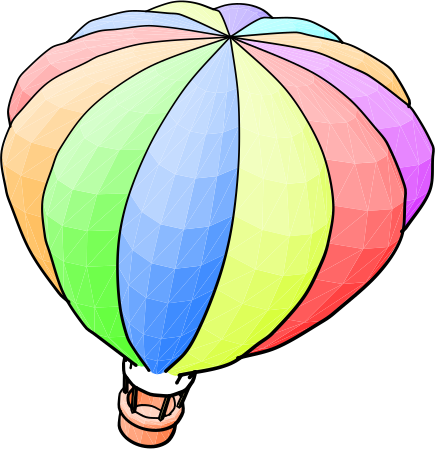
\includegraphics[width=3cm,height=3cm,keepaspectratio]{figures/smalltalk.pdf}%
					}%
				}%
			%}%
		\fi%
	}
}{}

\begin{document}
\frontmatter

\maketitle
% !TEX root = semexp-thesis.tex

\begin{abstract}
	TODO: abstract
\end{abstract}

\renewcaptionname{ngerman}{\abstractname}{Abstract (German)}
\begin{zusammenfassung}
	TODO: German abstract
\end{zusammenfassung}

% !TEX root = semexp-thesis.tex

\begingroup
\let\raggedsection\centering

\chapter*{Acknowledgments}
\label{cha:acknowledgments}
\endgroup
\begin{quotation}
	\noindent TODO: acks

	\ParSep

	Parts of this work will be published and presented at the ACM SIGPLAN International Symposium on New Ideas, New Pa\-ra\-digms, and Reflections on Programming and Software (Onward!~'24)~\cite{thiede2024talking}.
\end{quotation}

\cleardoublepage
% !TEX root = semexp-thesis.tex

\noindent
\begingroup
	%\footnotesize
	If you require a fully accessible version of this document, please contact me at \href{mailto:christoph.thiede@student.hpi.de}{christoph.\allowbreak thiede@\allowbreak student.hpi.de}.
\endgroup

% TODO: add copyrights page + merge it with this?

\cleardoublepage
\tableofcontents
%\listoffigures
%\listoftables
{\sloppy\listoffiguresandtables}
%\lstlistoflistings
%\listofacronyms %
\mainmatter
\thimport[chapters]{01_introduction}
\thimport[chapters]{02_background}
\thimport[chapters]{03_approach}
\thimport[chapters]{04_design}
\thimport[chapters]{05_suggestions}
\thimport[chapters]{06_agent}
\thimport[chapters]{07_implementation}
\thimport[chapters]{08_application}
\thimport[chapters]{09_discussion}
\thimport[chapters]{10_related_work}
\thimport[chapters]{11_conclusion}


\clearpage
\appendix
% !TEX root = semexp-thesis.tex

% \part{Appendix}
% \label{part:appendix}

\thimport[appendixes]{a_semtex}
\thimport[appendixes]{b_conversation}

%\printbibliography[heading=bibintoc]
\chapter*{Bibliography}
\addcontentsline{toc}{chapter}{Bibliography}
\markboth{Bibliography}{Bibliography}
\defbibheading{subbibliography}{%
	\section*{#1}
	\markboth{Bibliography}{#1}
	\pdfbookmark[2]{#1}{bibliography.#1}
}
\printbibliography[heading=subbibliography, title={Programming and Software Engineering}, keyword=bib-regular]
\printbibliography[heading=subbibliography, title={Artificial Intelligence and Machine Learning}, keyword=bib-ai]
\backmatter
\markboth{}\relax

\newbool{swastatement}
\setbool{swastatement}{false}
\ifbool{swastatement}{%
	% BAMA-O (2023) §30.6
	%  Am Schluss der Arbeit hat die Kandidatin bzw. der Kandidat zu versichern,
	%  dass sie bzw. er die Arbeit selbstständig verfasst und keine anderen
	%  Quellen und Hilfsmittel als die angegebenen benutzt hat.
	%\makeatletter
	%\gdef\statementcontent{%
	%	Hiermit versichere ich, dass ich die vorliegende Arbeit selbständig verfasst sowie ausschließlich angegebene oder zulässige Quellen und Hilfsmittel benutzt habe.
	%}
	%\makeatother
	% english
	\makeatletter
	\gdef\swa@statementname{Declaration of Authorship}
	\gdef\statementcontent{%
		I hereby certify that I have written this thesis independently and have used only the sources and tools indicated or permitted.
	}
	\pdfbookmark{Declaration of Authorship}{doa}\defaultstatement

	\noindent\\
	This document has been published digitally and is valid without a signature.
}{}

\end{document}
